\subsubsection{DNA and Chromosomes} \label{background:biology:dna_and_chromosomes}
\textit{Deoxyribonucleic acid} (DNA) is a polymer of two strands of nucleotides forming a double helix. 
It carries the genetic information making up the genome for all known organisms. 
The simplest building block composing the two DNA strands are \textit{nucleotides}.
The DNA strands are composed of long chains of four different nucleotides: cytosine, guanine, adenine and thymine, typically referred to as simply C, G, A and T respectively.
Furthermore, the two strands of DNA forming a double helix structure contain the same genetic information because they are complements of each other.
By examining one strand, the other can be determined by computing the complement of the first.
This is achieved by utilizing the base pairing rules, stating that A pairs with T and C pairs with G, forming the base-pairs AT/TA and CG/GC (a pairing of two nucleotides making up a position in the double helix connecting the two DNA strands).

DNA is organized into structures called chromosomes. 
Humans have 46 chromosomes made up by two sets of 23 chromosomes where each chromosome occurs twice, whereas one is inherited from the male parent and the other is inherited from the female parent.

\begin{figure}[ht!]
\begin{center}
\scalebox{1}{
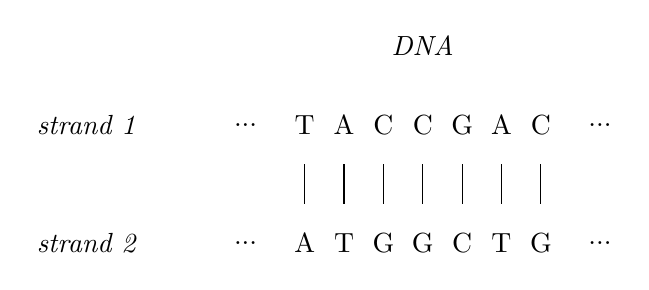
\begin{tikzpicture}

  \node at(2.25,2.5)(title){\textit{DNA}};
  \node at(-2,0)(title){\textit{strand 2}};
  \node at(-2,1.5)(title){\textit{strand 1}};

  % Nodes
  \node at(0,0)(n1){...};
  \node at(0.75,0)(n2){A};
  \node at(1.25,0)(n3){T};
  \node at(1.75, 0)(n4){G};
  \node at(2.25,0)(n5){G};
  \node at(2.75,0)(n5){C};
  \node at(3.25,0)(n5){T};
  \node at(3.75,0)(n5){G};
  \node at(4.5,0)(n5){...};

  \node at(0,1.5)(n1){...};
  \node at(0.75,1.5)(n2){T};
  \node at(1.25,1.5)(n3){A};
  \node at(1.75,1.5)(n4){C};
  \node at(2.25,1.5)(n5){C};
  \node at(2.75,1.5)(n5){G};
  \node at(3.25,1.5)(n5){A};
  \node at(3.75,1.5)(n5){C};
  \node at(4.5,1.5)(n5){...};

  % base pair connects
  \draw (0.75,0.5) -- (0.75,1);
  \draw (1.25,0.5) -- (1.25,1);
  \draw (1.75,0.5) -- (1.75,1);
  \draw (2.25,0.5) -- (2.25,1);
  \draw (2.75,0.5) -- (2.75,1);
  \draw (3.25,0.5) -- (3.25,1);
  \draw (3.75,0.5) -- (3.75,1);

\end{tikzpicture}
}
\caption{A conceptual representation of two DNA strands composed of nucleotides forming base pairs where A (adenine) and T (thymine), and C (cytosine) and G (guanine) are complements of each other.}
\label{background:biology:dna_and_chromosomes:figures:dna_strands}
\end{center}
\end{figure}
